\documentclass{scrartcl}
\usepackage{minted}
\usepackage{fontspec}
\usepackage{makeidx}
\usepackage{listings}
\usepackage{graphicx}
\usepackage[colorlinks]{hyperref}
\setcounter{tocdepth}{5}

\title{Spock -{} Publish/subscribe framework for the Netduino}
\author{Franklin\textsc{Delehelle}}
\date{}
\makeindex
\makeglossary

\begin{document}
\maketitle
\newpage
\tableofcontents
\newpage

\begin{abstract}
~\\ \vspace{3cm} \begin{center} \textit{\large Abstract} \end{center} \vspace{1cm}

This report describes the objectives, development and result of the development of a publish/subscribe framework for
applications running on a network of netduinos and needing to exchange data.  \vspace{0.3cm}

We'll explain why we decided to use the publish/subscribe architecture, then see how we implemented a meshed
architecture, allowing a resilient network.  \vspace{0.3cm}

Then, we'll explain how we used both the TCP and UDP protocol to satisfy to our earlier requirements.  \vspace{0.3cm}

Thereafter, we'll detail the problematic of the exchange of the objects, the choice of the serialization method end how
the limitations of the netduino devboard leaded us toward a working but non optimal solution.  \vspace{0.3cm}

Finally, we'll see how to use the middleware and explain why we felt the need to develop a new one instead of using an
existing and hardened one.  \vspace{0.3cm}

\end{abstract} \newpage

\section{Introduction}

\subsection{Motivation}

Allowing distributed applications to share data safely and efficiently is not always an easy thing.  For this goal, the
data exchange utilities are gathered together in a middleware responsible for carrying the foresaid data amongst all the
running applications that need them. This middleware is also responsible for ensuring that the needed data are delivered
to the applications that need it, whether on the same board or an other one, by abstracting the transport layer.

\subsection{Architecture}

\subsubsection{General design}

A classic architectural pattern to satisfy to this constraints is the publish/subscribe architecure.  The
publish/subscribe type of middleware answers to the foresaid constraints by introducing to kind of agents.

The first one, the \textbf{publisher}, is a \emph{producer} of data. Its comportment is quite simple: each time it wants
to share data, it send them to the middleware.  Then, this one will guess the type of the data, then delivers them to
the concerned subscribers

The second one, the \textbf{subscriber}, is a \emph{consumer} of data. Its first action is to apply for a specific kind
of data to the middleware. The, each time a corresponding data is published to the middleware, this one will notify the
publisher of the event by triggering a callback method, allowing the subscriber to process the newly received data.
Then, when it doesn't need a type of data anymore, the subscriber has to tell it to the middleware. So, it'll be removed
from the list of programs needing this kind of data and won't be triggered anymore when new data are available.

Generally, this kind of service is ensured by a centralized server, for instance in JMS, the \emph{Java messaging
service}, but here we need to have a resilient system, which have to work even if a random node is diconnected from the
network. So, we have to implement a decentralized architecture, where every node can simultaneously be a server and a
client, depending on what the programs running on the node need.

\subsubsection{Advantages}

The advantages of this solution are mutiple. Neither the publishers nor the subscribers need to bother with the
communication between them as everything is managed by the middleware; they could be on the same board or in different
buildings, it doesn't matter. So, the ease of development for the people using the system is greatly increased by the
full abstraction of the spatial repartition of all the nodes.

Also, the middleware is running in other threads than the application, so the program isn't annoyed by the thread
management as the work of the middleware is transparently asynchronous. Moreover, as main part of the work -{} whether
the temporary storage or the dipatching of the data -{} is asynchronously done by the middleware, publishers and
subscribers are temporally fully independant.

Eventually, a tight synchronization between all of the publishers and subscribers isn't necessary. A subscriber can
enter the middleware after the subscribers offering the type of data it needs, it will still able to collect the type of
data it needs, because the middleware take care to optimize the repartition of the published data to all the publishers
connected to the middleware.

\pagebreak[4]


\section{Implementation}

\subsection{Current state}

Currently, the middleware offers a meshed network of nodes, each of them being publisher, subscriber or both depending
of the use of the library by the programs running on the board.

There is a singleton instance, which is designed to be thread safe, of the \texttt{Node} class running on each board,
and process publishing and subscribing both for program running on the same board as for nodes running on other boards
connected on an IPv4 network.

The library can work indifferently on the .NET MF or on the Mono platform. So, it is also usable between standard
desktop computers (certified tested at home). And it can be used on any platform supporting Mono, whether *BSD,
GNU/Linux, Windows or OS X.

\subsection{Data transmission}

One of the main point of a publish/subscribe middleware is to chose a format to encode the data exchanged between the
actors.

\subsubsection{The fellowship of the serialization}

At first, we wanted to use the \href{http://code.google.com/p/protobuf/}{Google protobuf} protocol for several reasons.
First of all, the protocol is already existing and well designed, which is a good start for a protocol. Second, it is
widely used in a whole range of products. And finally, there are implementations for a lot of languages, amongst them
C++, Java, python, C\#, \ldots{}

So, we could have been able to exchange the binary data between the devboards and a lot of other platforms, as long as
they could run one of these multiple implementations.

\subsubsection{The two frameworks}

There are two libraries implementing the protobuf protocol in .NET. The first one is
\href{http://code.google.com/p/protobuf-net/}{protobuf-{}net} and the second one is
\href{http://code.google.com/p/protobuf-csharp-port/}{protobuf-{}csharp-{}port}.

The first one is able to serialize a .NET object on the fly without the \texttt{.\penalty0 proto} corresponding file
thanks to its intensive use of the introspection capabilities of the .NET stack. However, it's not compatible with other
implementations as its doesn't use these \texttt{.\penalty0 proto} files.

The second one is a more orthodox implementation of the protobuf protocol and seems to stick to the norm. It's using
\texttt{.\penalty0 proto} file to generate C\# classes that contains methods to be serialized through the protobuf
protocol into binary streams or XML files.

So, both of these librairies where really intersting, the first one to easily exchanges objects between .NET only
applications, and the second one to exchange data with any platform running an implementation of the protobuf protocol,
to the cost of a little more difficult use and the need to write the \texttt{.\penalty0 proto} specification files.
Also, as the classes are automatically generated, you can't heavily customize them.

However, the netduinos are running the microframework, which is a
\href{http://www.flickr.com/photos/22221147@N02/2223126904/}{clipped, clapped, cropped} version of the whole .NET
framework. And it happens that amongst other limitations, the .NET MF support neither the generics objects nor the whole
introspection library. So, as the first one need introspection ond the second one generics, both of them weren't usable
on the .NET MF, which is regrettable.

\subsubsection{The return of the Solution}

Eventually, we decided to use the classic .NET serialization for the exchange of objects between the netduinos. Of
course, it's not as efficient and versatile as protobuf, but at least it works on the .NET MF.

To be able to exchange objects with other applications running the real protobuf protocol, we want to design a gateway
between the subnetwork of the netdinos and the subnetwork of the machines using the true .NET framework, designed to use
the \texttt{pro\penalty5000 t\penalty5000 o\penalty5000 buf-{}\penalty0 net} library to convert serializable objects to
protobuf-{}serialized objects. So, the two protocols will be able to cooperate on the same network.  And this is
achievable because protobuf-{}net is able, thanks to its intensive use of introspection, to serialize objects to the
protobuf protocol on the fly, allowing us to easily share .NET objects.

However, as the serialization algorithms aren't the same ont the full-{}fledged .NET framework and on the .NET MF, a
little more work will be required to deserialize the objects received by the proxy from the netduinos. So it could be
interesting to implements our own methods of serialization and deserialization.

\subsection{Network layer}

I wanted to do a framework as resilient as possible and able to support random connection or deconnection of the nodes.
So, I decided to use both the TCP and UDP protocols to reach this goal, the first one for autodiscovery and requests,
the second one for transmission of the objects and peer to peer communications.

\subsubsection{Network layout}

Currently, the network layout is "everybody is connected to everybody he needs to speak". As there is no real hierarchy
in the netduino networks and that, communication being done overt ethernet, there is no need for multi-hop energy
saving, the need for a more refined architecture didn't come up.

\subsubsection{Configuration}

The network layer slightly support customization by modifying the constants in the beginning of \texttt{Nod\penalty5000
e\penalty5000 N\penalty5000 e\penalty5000 t\penalty5000 w\penalty5000 o\penalty5000 r\penalty5000 k\penalty5000
L\penalty5000 a\penalty5000 yer.\penalty0 cs}. They are :

\noindent \begin{description} \item[{ UDP\_PORT }] \hspace{0em}\\ the port used for UDP communications

\item[{ TCP\_PORT }] \hspace{0em}\\ self-{}explanatory\ldots{}

\item[{ TCP\_MAX\_TRIES }] \hspace{0em}\\ the max number of tries when sending something to an other node

\item[{ TCP\_TIMEOUT }] \hspace{0em}\\ the max delay for trying to establish a TCP communication with an other node

\item[{ ourIP }] \hspace{0em}\\ theorically, it is designed to use either the ethernet interface on netduino or the
	second interface on desktop (the first one being the local loop), but it could need to be modified for more complex
	systems.

\end{description}

\subsubsection{UDP usage}

As foresaid, UDP is used for the discovery of interesting peers. Why UDP ? Simply because I need broadcast and TCP only
give me uni-{} and multicast (and yet, every device on the route must be compatible with it, which is not oftn the
case), so goodbye TCP, welcome UDP.

I'd say that I'm using it a little overwhelmingly, but at least it just works.

The method processing UDP connections is \texttt{lis\penalty5000 t\penalty5000 e\penalty5000 n\penalty5000 F\penalty5000
o\penalty5000 r\penalty5000 U\penalty5000 D\penalty5000 P\penalty5000 R\penalty5000 e\penalty5000 q\penalty5000
u\penalty5000 e\penalty5000 sts}, in \texttt{Nod\penalty5000 e\penalty5000 N\penalty5000 e\penalty5000 t\penalty5000
w\penalty5000 o\penalty5000 r\penalty5000 k\penalty5000 L\penalty5000 a\penalty5000 yer.\penalty0 cs}.

\noindent
\begin{description}
\item[{ UDP\_COMMAND\_ASKSFOR }] \hspace{0em}\\
First, each time a subscriber subscribes to something, it broadcasts an offering datagram. Each node publishing the needed kind of data stores the IPv4 address of the broadcaster and will send it corresponding data next time one of its publishers delivers it.

\item[{ UDP\_COMMAND\_OFFERS }] \hspace{0em}\\ Also, \emph{each time} a node receive an object to publish, it broadcasts
	an offer message for two reasons. First, to inform subscriber that where whether not interested or not connected at
	the first offer, and second, in the case where previous datagrams were lost (UDP\ldots{} what did you expect ?).

\item[{ UDP\_COMMAND\_DOESNTNEED }] \hspace{0em}\\ Finally, when a node receive an unsubscribe request and there is only
	one local subscriber, it broadcast a datagram to let everyone know on the network that it doesn't need this kind of
	objects anymore.

\end{description}

\subsubsection{TCP usage}

The TCP is used whenever we need node to node communication thanks to its reliability. More precisely, it is used in two
cases.

The method processing TCP connections is \texttt{lis\penalty5000 t\penalty5000 e\penalty5000 n\penalty5000 F\penalty5000
o\penalty5000 r\penalty5000 T\penalty5000 C\penalty5000 P\penalty5000 R\penalty5000 e\penalty5000 q\penalty5000
u\penalty5000 e\penalty5000 sts}, in \texttt{Nod\penalty5000 e\penalty5000 N\penalty5000 e\penalty5000 t\penalty5000
w\penalty5000 o\penalty5000 r\penalty5000 k\penalty5000 L\penalty5000 a\penalty5000 yer.\penalty0 cs}.

\noindent
\begin{description}
\item[{ TCP\_COMMAND\_ACCEPT\_TYPE }] \hspace{0em}\\
when a node receive the information of the presence of an interesting data type over UDP broadcast, it extracts the sender IP from the datagram and contact it over TCP to tell it it's interested in what it has to offer.

\item[{ TCP\_COMMAND\_OBJECT }] \hspace{0em}\\
whenever a node has to send a serialized object to another one, it establishes a TCP connection and send it the object with the foresaid opcode.

\end{description}

\subsubsection{Example}

\begin{figure} 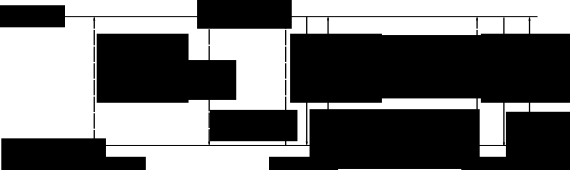
\includegraphics{graph.pdf} \caption{UDP datagram are in dashed arrows, TCP transmission in plain}
\end{figure}

You can see on figure 1 that a subscriber (on node 1) came after an interesting publisher (on node 2). So, when the
publisher received the UDP broadcast asking for data, it sends the corresponding data (throught TCP).

However, even if the TCP communications sending objects seem to be a response to the TCP communications accepting the
data type, they're not, it's just that they happen roughly at the same time.

Indeed, the publisher emits the offer at each publication in case there was an interested subscriber that wheter asked
for this kind of data berfore the publisher went online or in case of lost UDP datagram. But still, the subscriber emits
an "asks for" datagram, so it doesn't have to register \emph{after} the first object emission, and so, miss it.

\pagebreak[4]


\section{The netduino}

I wanted to dedicate a section to the development on the netduino, because it was an important part of the project, and
I think that this devboard is really interesting by the contrasts it has to offer.

However, I'd like to say that I'm a Linux user and a fan of vim, in terminal compilation and other lightweight tools, so
I'm of course influenced by my background.

\subsection{Development on the netduino}

To develop on the netduino, one must install Visual Studio 2010, it's dependencies, and then the microframework SDK for
the netduino. And after this has been done, I was surprised to see that I needed several gigabytes of software -{}
including an SQL server -{} to develop on a little devboard.

On a second thought, I was suprised that the SDK was only available for a four years old version of Visual Studio.
However I'm not sure that I didn't miss a more recent version of the SDK.

I have only two relevant comments on Visual Studio itself: first, the color theme is horrible and I didn't managed to
easily change it; second, the IntelliSense is just great, I think it's one of the best and fastest auto-{}completion
engin I ever saw besides KDevelop's one.

\subsection{The .NET platform}

First of all, I have to say that having the comfort of development .NET framework was a pleasure. I never used C\#
before -{} only C++ and Java -{}, but the language in itself, despite a few archaisms (the scope of the \texttt{case}
for instance), was a real pleasure to use

I also discovered some new concepts existing neither in C++ nor in Java that were nice to use. I really appreciated the
partial classes, which allowed me to split huge classes in several files. I know that it's possible in C++ , but I found
the C\# implementation to be quite clean and handy.

Also, the system of properties is just wonderful. It allows to use the security of the encapsulation with the ease of
use of simple attributes. I know it's only syntactic sugar, but after all, isn't just C syntactic sugar for assembly ?
So yes, I'm fond of C\#'s properties.

And, more generally, the standard library is just \textbf{colossal}. I know that we're used to this with
"not-{}so-{}recent" platforms (JVM and .NET mainly), but it's often a pleasure, when you look for a functionality, to
see that there is a canonical implementation of it in the standard library of the language you're using.

\subsection{The microframework}

However, the microframework is something else\ldots{} the idea is fine, but the realization is disappointing. There are
three main things that I find really disappointing on the microframework.

\subsubsection{The generics}

The lack of generics in the .NET MF is a shame. Generic types are a killer feature of high level language (mainly
because they offer a stronger typing), and having C\# amputated of this feature is really frustrating.

I understand that C\# generics are computed at runtime and so use some processing power and so could be too heavy for
the Atmel of the netduino, but they could have implemented generics \emph{� la} C++.

With this process, the instantiation of a generic class generate the source code needed for this instance of the
generic, meaning that instantiating for example a \texttt{vec\penalty5000 t\penalty5000 o\penalty5000 r\penalty5000
<{}\penalty5000 i\penalty5000 nt>{}} will generate the source code for a \texttt{vec\penalty5000 t\penalty5000
o\penalty5000 r\penalty5000 \_\penalty5000 int} class with all the methods using \texttt{int} parameters.

This method is probably heavier in overall than the .NET method, but the work is done by the compiler during the build
of the program, so it'd allow us to use the generics on the netduino without overloading its CPU., which would be a win
for us.

\subsubsection{Introspection}

The absence of advanced introspection is really a pity. Technically speaking, I understand better this problem then the
generics' one because the Atmel isn't really a power beast and we need to run actual programs on the board. But I have
to confess that I think that removing introspection blows up one of the main advantage of managed languages (with memory
management, but we're responsible adults and we absolutely never have segfaults and memory leak, don't we ? ;) over
compiled language.

\subsubsection{Standard library}

But still, in spite of these deceptions, the microframework offers a \textbf{huge} library, and it's wonderful.

Compared to devboard running a small realtime OS, it's really a great thing to develop practically like on your desktop.
But if the MS guys could just implements a few more things, it'd be just great.

For instance, during this project, I had to find an alternative implementation of the byte array to native type
transformation. As it's in the official .NET library, I don't understand why it's not in the .NET MF. There are no
technical problems, it's just a few bitwise operations and a couple of casts !

Also, why isn't the class \texttt{Tcp\penalty5000 L\penalty5000 i\penalty5000 s\penalty5000 t\penalty5000 e\penalty5000
ner} there ? Ok, it's just syntaxic sugar for \texttt{Soc\penalty5000 ket}, but why don't add it ?

\subsubsection{Conclusion}

It's really a shame to see that there are only these two big lack, introspection and generics, that makes the .NET MF a
nice development environment instead of a real great experience allowing to easily port whatever .NET program to the
netduino.


\pagebreak[4]


\section{Usage}

As said before, Spock is designed to run with only a singleton on each node. So, everytime that someone wants to use the
middleware, he has to get the singleton first.

\subsection{As a publisher}

Here is a little commented example on how to use Spock as a publisher.

\begin{minted}[mathescape,numbersep=5pt,fontsize=\footnotesize,frame=lines,framesep=2mm]{csharp}
using System;
#if MF
using Microsoft.SPOT;
#endif
using System.Diagnostics;

namespace Spock
{
    class TestPublisher
    {
        public static void test()
        {
            try
            {
                Node node = Node.Instance; // Get the singleton
                int i = 0;

                while (true)
                {
                    node.publish("KIKOOLOL #" + i++); // Publish a string
                    System.Threading.Thread.Sleep(1000); // Do whatever you want
                }
            }
            catch (Exception e)
            {
                Debug.Print(e.Message);
                Debug.Print(e.StackTrace);
            }

        }
    }
}
\end{minted}

In fact, the core of the program is this line:

\begin{minted}[mathescape,numbersep=5pt,fontsize=\footnotesize]{csharp}
node.publish("KIKOOLOL #" + i++); // Publish a string
\end{minted}

From here, Spock will find what kind of type the publisher wants to share and dispatch it to all the
concerned subscribers.

\pagebreak[4]


\subsection{As a subscriber}

Here is now what a subscriber's code looks like.

\begin{minted}[mathescape,numbersep=5pt,fontsize=\footnotesize,frame=lines,framesep=2mm]{csharp}
using System;
using System.Threading;
#if MF
using Microsoft.SPOT;
#endif
using System.Diagnostics;

namespace Spock
{
    class TestSubscriber : ISubscriber
    {
        public void test()
        {
            try
            {
                Node node = Node.Instance;

                Debug.Print("Subscribing to string");
                node.subscribe("".GetType(), this);

                Thread.Sleep(3000);

                Debug.Print("Unsubscribing to string");
                node.unsubscribe("".GetType(), this);
            }
            catch (Exception e)
            {
                Debug.Print(e.Message);
                Debug.Print(e.StackTrace);
            }
        }

        public void receive(Object o)
        {
            Debug.Print("Receiving an object of type " + o.GetType().Name);
        }
    }
}
\end{minted}

As before, with the publisher, we first need to obtain a reference to the singleton :

\begin{minted}[mathescape,numbersep=5pt,fontsize=\footnotesize]{csharp}
Node node = Node.Instance;
\end{minted}

Then, we have to subscribe to the type of data which is interesting us, currently the \texttt{Str\penalty5000 ing}.

\begin{minted}[mathescape,numbersep=5pt,fontsize=\footnotesize]{csharp}
node.subscribe("".GetType(), this);
\end{minted}

As we implements the \texttt{ISu\penalty5000 b\penalty5000 s\penalty5000 c\penalty5000 r\penalty5000 i\penalty5000 ber}
interface, the method \texttt{voi\penalty5000 d r\penalty5000 e\penalty5000 c\penalty5000 e\penalty5000 i\penalty5000
v\penalty5000 e\penalty5000 (\penalty5000 O\penalty5000 b\penalty5000 j\penalty5000 e\penalty5000 c\penalty5000 t o)}
will be called by Spock when it gets something that's intersting us. And that's what we say when we pass \texttt{this}
as the \texttt{ISu\penalty5000 b\penalty5000 s\penalty5000 c\penalty5000 r\penalty5000 i\penalty5000 ber} to notify.

Here, we're only registered for \texttt{Str\penalty5000 ing}. However, if we were registered for multiple types, we
would have to cast the received objects accordingly to what we expect.

\newpage \section{Conclusion}

\subsection{Related work}

\subsubsection{Canonical solutions}

Classicaly, one wanting to use a middleware to share data across a network will use piece of software like Microsoft's
DCOM or other messaging middleware available on the .NET platform, such as Mass Transit or Univeral messaging.

However, there are three points that prevented us to use one of them:
\begin{description}
	\item[.NET MF] none of them is able to run on the .NET MF, due to the lack of generics and/or introspection
	\item[netduino] the netduino is a small embedded device, so it can't support the weight of a full-fledged
	enterprise-dimensioned framework
	\item[flexibility] we needed a decentralized middleware, but all of these frameworks are working with a centralized architecture, therefore they weren't usable in our case
\end{description}


\subsubsection{Related researches}

A powerful middleware is described by \textsc{Rinner, Jovanovic \& Quaritsch}\footnote{\emph{Embedded middleware on
distributed smart cameras}}. It allows, amongst other functionalities, to distribute and execute different programs on
the fly, so that each camera in the network can be reconfigured to an other purpose. It's really a big thing for dynamic
distributed computing. However, this technology is too heavy for the netduino, and the only part that intersests us in
the case, i.e.\ the network communication module, is only a portion of the whole framework.

\href{http://www.codeproject.com/Articles/655774/Ella-publish-subscribe-middleware}{Ella}\footnote{\emph{Ella:
Middleware for Multi-camera Surveillance in Heterogeneous Visual Sensor Networks}} is a similar publish/subscribe
middleware developed by Bernhard \textsc{Dieber} and Jennifer \textsc{Simonjan} at the Klagenfurt University. At the
beginning, it was supposed to be used, erasing the need to develop a new middleware as spock.However, this piece of
software was victim of it power: it needed too much functionalities to run on the netduino board.

Developed at Politecnico di milano, REDS\footnote{\emph{Content-based Publish-Subscribe in a mobile environment}} is a
Java publish/subscribe middleware oriented towards mobile devices. But not only there is no JVM running on the netduino,
but the very architecture of this projet isn't adapted to our needs. The lot of resources involved in routing, mobile
and wireless networks relative problematics make it irrelevant in our case.

There is also GREEN\footnote{\emph{GREEN: A Configurable and Re-configurable Publish-Subscribe Middleware for Pervasive
Computing}}, developed at the Lancaster University. GREEN is a highly configurable publish/subscribe framework. It's
designed to run on pervasive devices using heterogeneous wireless networks. Even if it's a really well designed
middleware, it's not usable in our case for several reasons. First, it's not runnin on the .NET MF. Second, it's not
fully decentralized. And, finally, it's using the classical topics/channels scheme, and therefore doesnt' use the
serialization/deserialization and transission of native objects as we're doing.


\subsection{What next?}

\subsubsection{For the project}

What's still to do on the project is, in first place, the proxy between .NET MF serialization and standard protobuf
objects. And as .NET MF's serialization isn't the same as the standard .NET framework's one, it will require a little of
low-level work (beware of the endianness).

Furthermore, I didn't have enough computers and devboard to extensively test Spock. So, writing a serie of unit tests
and launch it on a dozen of machines would be good to ensure that it works and scales correctly.

Also, it would be fine to take brutal deconnections into account. For now, a brutal deconnection will result into a
timeout each time a node will try to send something to the disonnected node. It'd be nice to count the numbers of failed
TCP transmission and consider the node as dead after a few.

And finally, a higher parallelisation would be a nice feature. However, it'd require tests to check how the .NET MF on
the netduino can scale its threads number.


\subsubsection{For the netduino}

I have no idea if it's in the domain of the laboratory, but I think that adding a real instrospection to the .NET MF
would be wonderful. Introspection is one of the killer feature of managed languages over native ones, so I'm sure a lot
of people would be very happy if such a feature was to appear.

Also, I think that some new additions to the .NET MF standard library would be easy to add and really helpful.

Finally, it'd be really great if the society producing the netduino could finish the mono SDK, which is in alpha for
years, to allow us to develop on GNU/Linux, BSD or OS X.


\end{document}
